% Raphaël Heng : 23/09/22
\chapter{Fonctions réelles}
\section{Fonctions}

\begin{graybox}
	\begin{definition}[Fonction]
		Une fonction est la donnée de :
		\begin{itemize}
			\item Un ensemble de départ E
			\item Un ensemble d'arrivée F
			\item Une flèche : $f : E \to F$ à tout élément $x \in E$ associe un élément $f(x) \in F$
		\end{itemize}
	\end{definition}
\end{graybox}

\begin{exemple}
	\begin{align*}
		f_1 : 
		\begin{cases}
			\R &\to \R \\
			x &\mapsto 2x + 3
		\end{cases}
	\end{align*}
	\begin{align*}
		f_2 : 
		\begin{cases}
			\R^{*} &\to \R^{*} \\
			x &\mapsto \frac{1}{x}
		\end{cases}
	\end{align*}
	\begin{align*}
		f_3 : 
		\begin{cases}
			\R^{*} &\to \R \\
			x &\mapsto \frac{1}{x}
		\end{cases}
	\end{align*}
	\begin{align*}
		\mid \cdot \mid : 
		\begin{cases}
			\R &\to \R \\
			x &\mapsto 
			\begin{cases}
				x \textnormal{ si } x \geq 0 \\
				-x \textnormal{ si } x < 0
			\end{cases}
		\end{cases}
	\end{align*}
\end{exemple}

\begin{remarque}
	$f_2 \neq f_3$ car leurs ensembles d'arrivée sont différents.
\end{remarque}

\begin{remarque}[Vocabulaire]
	Si $f : E \to F$ est une fonction, on appelle parfois l'ensemble de départ E, le domaine de $f$ et l'ensemble d'arrivée F, le codomaine de $f$.
\end{remarque}

\begin{remarque}
	Lorsque que $E = F = \R \textnormal{ ou une partie de } \R$, on parle de fonction réelles. 
\end{remarque}


\subsection{Produit cartésien et graphe}

\begin{graybox}
	\begin{definition}[Produit cartésien]
		Si E et F sont deux ensembles, on appelle $E \times F$ leur produit cartésien.
		\begin{align*}
			E \times F = \{(x, y),\ x \in E,\ y \in F\}
		\end{align*}
	\end{definition}
\end{graybox}

\begin{remarque}
	On écrit $E^2 \text{ plutôt que } E \times E$
\end{remarque}

\begin{graybox}
	\begin{definition}[Graphe d'une fonction]
		Si $f : E \to F$ est une fonction, son graphe est défini comme 
		\begin{align*}
			Gr(f) = \{(x, f(x)),\ x \in E\} \subset E \times F
		\end{align*}
	\end{definition}
\end{graybox}

\begin{remarque}
	Le graphe d'une fonction réelle $f : \R \to \R$ est une partie de $\R^2$. On peut le dessiner.
\end{remarque}

\begin{remarque}
	Une partie $A \subset \R^2$ est le graphe d'une fonction de $\R \to \R$ si et seulement si toute droite verticale intersecte A en un unique point.
\end{remarque}



\section{Fonctions injectives, surjectives et bijectives}

\begin{graybox}
	\begin{definition}[Image et antécédent]
		Soient E et F des parties de $\R$ et $f:E \to F$ une fonction.
		Si $x \in E$ et $y \in F$ vérifient $y = f(x)$ on dit que $y$ est l'\textbf{image} de $x$ par $f$ et que $x$ est un \textbf{antécédent} de $y$ par $f$.
	\end{definition}
\end{graybox}

\begin{remarque}
	Les articles "l'" et "un" sont importants. Chaque image peut avoir plusieurs antécédents mais un antécédent a au plus une image.
\end{remarque}

\begin{exemple}~
	\\
	Pour la fonction 
	$
	f :
	\begin{cases}
		\R &\to \R \\
		x &\mapsto x^2
	\end{cases}
	$
	\\ 
	$y = 4$ \textnormal{a deux antécédents} : $x = 2 \textnormal{ ou } x = -2$ mais $y = -4$  n'a pas d'antécédent.
\end{exemple}

\begin{graybox}
	\begin{definition}[Surjectivité]
		On dit qu'une fonction est \textbf{surjective} ou une \textbf{surjection} si tout élément de F admet \textbf{au moins} un antécédent par $f$.
		\begin{align*}
			\{\forall y \in F,\ \exists x \in E,\ y = f(x)\} \iff f : E \to F \textnormal{ est surjective }
		\end{align*}
	\end{definition}
\end{graybox}

\begin{exemple}~
	\\
	$
	f_1 : 
	\begin{cases}
		\R^* &\to \R \\
		x &\mapsto \frac{1}{x}
	\end{cases}
	$
	, n'est pas surjective, 0 n'a pas d'antécédent. 
	\\
	$
	f_2 : 
	\begin{cases}
		\R^* &\to \R^* \\
		x &\mapsto \frac{1}{x}
	\end{cases}
	$
	, est surjective, un antécédent de $y \in \R^*$ est $\frac{1}{y}$
\end{exemple}

\begin{remarque}~
	\\
	$\text{Soit } f : \R \to \R \text{ , f est surjective } \iff \text{ toute ligne horizontale rencontre le graphe } Gr(f)$ \\
\end{remarque}

\begin{graybox}
	\begin{definition}[Injectivité]
		On dit que $f : E \to F$ est \textbf{injective} (\textbf{une injection}) si tout élément de F admet \textbf{au plus} un antécédent par $f$.
		Ceci revient à dire : 
		\begin{align*}
			\text{ f injective } \iff \{\forall (x_1, x_2) \in E^2,\ f(x_1) = f(x_2) \implies x_1 = x_2 \}
		\end{align*}
		Ou encore :
		\begin{align*}
			\forall(x_1, x_2) \in E^2,\ x_1 \neq x_2 \implies f(x_1) \neq f(x_2)
		\end{align*}
	\end{definition}
\end{graybox}

\begin{remarque}
	Une fonction $f : \R \to \R$ est injective si et seulement si toute ligne horizontale rencontre $Gr(f)$ en 0 ou 1 point.
\end{remarque}

\begin{graybox}
	\begin{definition}[Bijectivité]
		Une fonction $f : E \to F$ est \textbf{bijective} (\textbf{une bijection}) si elle est \textbf{injective} et \textbf{surjective}. 
		\\
		Cela revient à dire que tout élément de F admet exactement 1 antécédent positif.
		\begin{align*}
			\text{f bijective} \iff \{\forall y \in F,\ \exists! x \in E,\ y = f(x)\}
		\end{align*}
	\end{definition}
\end{graybox}

\begin{graybox}
	\begin{definition}[Bijection réciproque]
		Lorsque $f : E \to F$ est une bijection. On peut définir :
		\begin{align*}
			f^{-1} :
			\begin{cases}
				F &\to E \\
				y &\mapsto \textnormal{ l'unique antécédent de } y
			\end{cases}
		\end{align*}
		La fonction $f^{-1}$ est une bijection, que l'on appelle bijection réciproque de $f$.
	\end{definition}
\end{graybox}

\begin{exemple}~
	\\
	Soit 
	$
	f : 
	\begin{cases}
		\R^+ &\to \R^+ \\
		x &\mapsto x^2
	\end{cases}
	$
	une fonction bijective. 
	\\
	Sa fonction réciproque est la fonction
	$
	f^{-1} :
	\begin{cases}
		\R^+ &\to \R^+ \\
		x &\mapsto \sqrt{x}
	\end{cases}
	$
\end{exemple}

\begin{remarque}
	Ne pas confondre réciproque et inverse, la fonction inverse de $f$ n'est pas $f^{-1}$ mais $\frac{1}{f}$
\end{remarque}

\begin{graybox}
	\begin{proposition}
		Si $f : E \to F$ est bijective, 
		\begin{align*}
			\forall x \in E,\ f^{-1}(f(x)) = x \\
			\forall y \in F,\ f(f^{-1}(y)) = y
		\end{align*}
	\end{proposition}
\end{graybox}


\section{Composition}

\begin{graybox}
	\begin{definition}[Composition de fonctions]
		Soient E, F, G des parties de $\R$ et $f: E \to F$ et $g: F \to G$.
		On définit la composée de $g$ par $f$, notée $g \circ f$ ("g rond f") comme :
		\begin{align*}
			g \circ f :
			\begin{cases}
				E &\to G \\
				x &\mapsto g(f(x))
			\end{cases}
		\end{align*}
	\end{definition}  
\end{graybox}  


\begin{remarque}
	La composée de $g \circ f$ n'est définie que si l'ensemble d'arrivée de $f$ est inclus dans l'ensemble de départ de $g$.
\end{remarque}

\begin{graybox}
	\begin{definition}[Fonction identité]
		On appelle fonction identité de E
		\begin{align*}
			id_E :
			\begin{cases}
				E &\to F \\
				x &\mapsto x
			\end{cases}
		\end{align*}
	\end{definition}
\end{graybox}

\begin{graybox}
	\begin{proposition}[]
		Si $f: E \to F$ est une bijection :
		\begin{align*}
			f^{-1} \circ f = id_E \\
			f \circ f^{-1} = id_F
		\end{align*}
	\end{proposition}
\end{graybox}

\begin{exemple}~
	\begin{align*}
		&f :
		\begin{cases}
			\R &\to \R \\
			x &\mapsto \sin{(x)}
		\end{cases}
		&g :
		\begin{cases}
			\R &\to \R \\
			x &\mapsto x + 2
		\end{cases}
	\end{align*}
	\begin{align*}
		&g \circ f :
		\begin{cases}
			\R &\to \R \\
			x &\mapsto \sin{(x)} + 2
		\end{cases}
		&f \circ g :
		\begin{cases}
			\R &\to \R \\
			x &\mapsto \sin{(x + 2)}
		\end{cases}
	\end{align*}
	\begin{align*}
		&f \circ f :
		\begin{cases}
			\R &\to \R \\
			x &\mapsto \sin{(\sin{(x)})}
		\end{cases}
		&g \circ g :
		\begin{cases}
			\R &\to \R \\
			x &\mapsto (x + 2) + 2 = x + 4
		\end{cases}
	\end{align*}
\end{exemple}


\section{Image directe, image réciproque}

\begin{graybox}
	\begin{definition}[Image directe]
		Soit $f : E \to F$ une fonction et A une partie de E.
		On définit l'image directe de A par $f$ comme :
		\begin{align*}
			f(A) = \{f(x), x \in A\},\ f(A) \subset F
		\end{align*}
	\end{definition}
\end{graybox}

\begin{graybox}
	\begin{definition}[Image réciproque]
		Si B est une partie de F. On décrit l'image réciproque de B par $f$ comme :
		\begin{align*}
			f^{-1}(B) = \{\forall x \in E,\ f(x) \in B\},\ f^{-1} \subset E
		\end{align*}
	\end{definition}
\end{graybox}

\begin{exemple}~
	\begin{align*}
		f:
		\begin{cases}
			\R &\to \R \\
			x &\mapsto x^2
		\end{cases}
	\end{align*}
	\begin{itemize}
		\item $f([1;2]) = [1;4]$
		\item $f^{-1}([-1;2]) = [-\sqrt{2};-1]\cup[1;\sqrt{2}]$
		\item $f(]-2;1[) = [0;4[$
		\item $f^{-1}(]-2;1[) = ]-1;1[$ 
	\end{itemize}
\end{exemple}

\begin{remarque}
	L'image réciproque $f^{-1}(B)$ est toujours définie même si $f$ n'est pas supposé bijective.
\end{remarque}

\begin{remarque}
	Si $f$ est bijective, l'ensemble $f^{-1}(B)$ est aussi l'image directe de B par $f^{-1}$
\end{remarque}


\clearpage

\begin{graybox}
	\begin{proposition}[Propriétés sur les images directes et réciproques]
		Soient $f:E \to F$ une fonction, $A_1 \subset E, A_2 \subset E$ et $B_1 \subset F, B_2 \subset F$
		\begin{itemize}
			\item $f(A_1 \cup A_2) = f(A_1) \cup f(A_2)$
			\item $f^{-1}(B_1 \cup B_2) = f^{-1}(B_1) \cup f^{-1}(B_2)$
			\item $f^{-1}(B_1 \cap B_2) = f^{-1}(B_1) \cap f^{-1}(B_2)$
		\end{itemize}
	\end{proposition}
\end{graybox}

\begin{remarque}
	La proposition $f(A_1 \cap A_2) = f(A_1) \cap f(A_2)$ est fausse.
	\\
	Contre-exemple : $A_1 = [1;2], A_2 = ]-2; 1[$ et 
	\begin{align*}
		f :
		\begin{cases}
			\R &\to \R \\
			x &\mapsto x^2
		\end{cases}
	\end{align*}
	\begin{itemize}
		\item $f(A_1) = [1;4],\ f(A_2) = [0;4[$
		\item $f(A_1) \cap f(A_2) = [1;4[$
		\item $A_1 \cap A_2 = \emptyset$
		\item $f(A_1 \cap A_2) = \emptyset$
		\item $\emptyset \neq [1;4[$
	\end{itemize}    
\end{remarque}


\section{Opérations sur les fonctions}
\noindent Soient $A \subset \R$ et $f:A \to \R,\ g:A\to \R$ deux fonctions

\begin{graybox}
	\begin{proposition}[Somme de fonctions]
		\begin{align*}
			f + g : 
			\begin{cases}
				A &\to \R \\
				x &\mapsto f(x) + g(x)
			\end{cases}
		\end{align*}
	\end{proposition}
\end{graybox}

\begin{graybox}
	\begin{proposition}[Produit de fonctions]
		\begin{align*}
			fg : 
			\begin{cases}
				A &\to \R \\
				x &\mapsto f(x)g(x)
			\end{cases}
		\end{align*}
	\end{proposition}
\end{graybox}

\begin{graybox}
	\begin{proposition}[Quotient de fonctions]
		Si $g(x) \text{ ne s'annule pas sur A } \iff g(A) \subset \R^*$
		\begin{align*}
			\frac{f}{g} : 
			\begin{cases}
				A &\to \R \\
				x &\mapsto \frac{f(x)}{g(x)}
			\end{cases}
		\end{align*}
	\end{proposition}
\end{graybox}

\section{Propriétés sur les fonctions}

\begin{graybox}
	\begin{definition}[Fonction majorée]
		Soit $I \subset \R$ et $f:I\to \R$. 
		On dit que $f$ est majorée sur I si l'ensemble $f(I)$ est majoré.
		\begin{align*}
			f \text{ est majorée sur I} \iff \exists m \in \R, \forall x \in I, f(x) \leq m
		\end{align*}
	\end{definition}
\end{graybox}

\begin{graybox}
	\begin{definition}[Fonction minorée]
		Soit $I \subset \R$ et $f:I\to \R$. 
		On dit que $f$ est minorée sur I si l'ensemble $f(I)$ est minoré.
		\begin{align*}
			f \text{ est minorée sur I} \iff \exists m \in \R, \forall x \in I, f(x) \geq m 
		\end{align*}
	\end{definition}
\end{graybox}

\begin{graybox}
	\begin{definition}[Fonction bornée]
		Soit $I \subset \R$ et $f:I\to \R$. 
		On dit que $f$ est bornée sur I si l'ensemble $f(I)$ est borné.
		\begin{align*}
			f \text{ est bornée sur I} \iff \exists (m_1, m_2) \in \R^2, \forall x \in I, m_1 \leq f(x) \leq m_2
		\end{align*}
	\end{definition}
\end{graybox}

\begin{graybox}
	\begin{definition}[Fonction croissante]
		Soit $f$ une fonction, on dit que $f$ est croissante si 
		\begin{align*}
			\forall(x,y) \in I^2,\ x \leq y \implies f(x) \leq f(y)
		\end{align*}
	\end{definition}
\end{graybox}

\begin{graybox}
	\begin{definition}[Fonction décroissante]
		Soit $f$ une fonction, on dit que $f$ est décroissante si 
		\begin{align*}
			\forall(x,y) \in I^2,\ x \leq y \implies f(x) \geq f(y)
		\end{align*}
	\end{definition}
\end{graybox}

\begin{graybox}
	\begin{definition}[Fonction monotone]
		On dit qu'une fonction est monotone si elle est croissante ou décroissante.
	\end{definition}
\end{graybox}

\begin{graybox}
	\begin{definition}[Fonction strictement croissante]
		Soit $f$ une fonction, on dit que $f$ est strictement croissante si 
		\begin{align*}
			\forall(x,y) \in I^2,\ x < y \implies f(x) < f(y)
		\end{align*}
	\end{definition}
\end{graybox}

\begin{graybox}
	\begin{definition}[Fonction strictement décroissante]
		Soit $f$ une fonction, on dit que $f$ est strictement décroissante si 
		\begin{align*}
			\forall(x,y) \in I^2,\ x < y \implies f(x) > f(y)
		\end{align*}
	\end{definition}
\end{graybox}

\begin{graybox}
	\begin{definition}[Fonction strictement monotone]
		On dit qu'une fonction est strictement monotone si elle est strictement croissante ou strictement décroissante.
	\end{definition}
\end{graybox}

\begin{remarque}~
	\begin{itemize}
		\item Une fonction est croissante si toute droite passant par deux points de son graphe a un coefficient directeur positif.
		\item Une fonction est décroissante si toute droite passant par deux points de son graphe a un coefficient directeur négatif.
	\end{itemize}
\end{remarque}

\noindent Supposons qu'un intervalle $I$ est symétrique, c'est-à-dire que :
\begin{align*}
	x \in I \iff -x \in I
\end{align*}

\begin{graybox}
	\begin{definition}[Fonction paire]
		On dit qu'une fonction $f:I\to \R$ est paire si :
		\begin{align*}
			\forall x \in I,\ f(x) = f(-x)
		\end{align*}
	\end{definition}
\end{graybox}

\begin{graybox}
	\begin{definition}[Fonction impaire]
		On dit qu'une fonction $f:I\to \R$ est impaire si :
		\begin{align*}
			\forall x \in I,\ f(-x) = -f(x)
		\end{align*}
	\end{definition}
\end{graybox}

\begin{remarque}
	Si $f$ est impaire alors $f(0) = 0$
\end{remarque}

\begin{graybox}
	\begin{definition}[Fonction T-périodique]
		Soit $T > 0$.
		Une fonction $f:\R \to \R$ est T-périodique si :
		\begin{align*}
			\forall x \in \R,\ \forall n \in \Z,\ f(x + nT) = f(x)
		\end{align*}
	\end{definition}
\end{graybox}

\section{Propriétés géométriques du graphe}
\noindent Soit $f:\R \to \R$
\begin{itemize}
	\item 
	$
	f_1 : 
	\begin{cases}
		\R &\to \R \\
		x &\mapsto f(x) + a,\ a \in \R
	\end{cases}
	$
	\\
	$Gr(f_1)$ se déduit de $Gr(f)$ par translation de vecteur $a \Vec{j}$, ($j$ est le vecteur unitaire de l'axe des ordonnées). 
	\begin{align*}
		(x,y) \in Gr(f_1) &\iff y = f_1(x) \\
		&\iff y = f(x) + a \\
		&\iff y - a = f(x) \\
		&\iff (x, y - a) \in Gr(f)
	\end{align*}        
	\begin{figure}[h!]
		\centering
		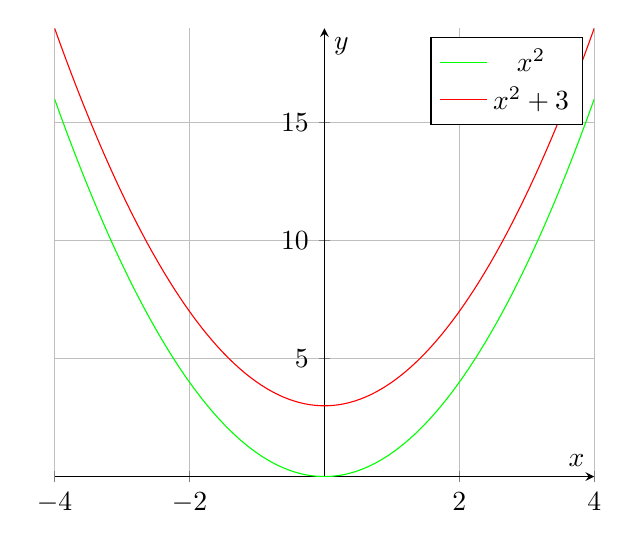
\begin{tikzpicture}
			\begin{axis}[domain=-4:4, axis lines=middle, grid=both, xlabel=$x$, ylabel=$y$, samples=100]
				\addplot[color=green]{x^2};
				\addlegendentry{$x^2$};
				\addplot[color=red]{x^2 + 3};
				\addlegendentry{$x^2 + 3$};
			\end{axis}
		\end{tikzpicture}
	\end{figure}
	
	\item
	$
	f_2 :
	\begin{cases}
		\R &\to \R \\
		x &\mapsto f(x+a),\ a \in \R
	\end{cases}
	$
	\\
	$Gr(f_2)$ se déduit de $Gr(f)$ par translation de vecteur $-a \Vec{i}$, ($i$ est le vecteur unitaire de l'axe des abscisses).
	\begin{align*}
		(x,y) \in Gr(f_2) &\iff y = f_2(x) \\
		&\iff y = f(x + a) \\
		&\iff (x + a, y) \in Gr(f)
	\end{align*}    
	\begin{figure}[h!]
		\centering
		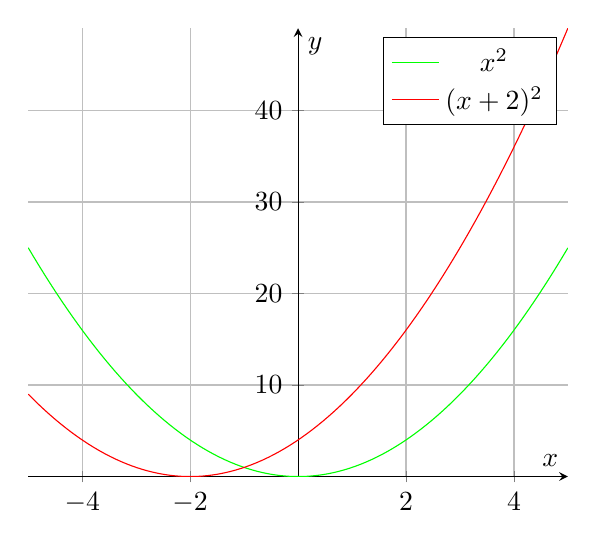
\begin{tikzpicture}
			\begin{axis}[domain=-5:5, axis lines=middle, grid=both, xlabel=$x$, ylabel=$y$, samples=100]
				\addplot[color=green]{x^2};
				\addlegendentry{$x^2$};
				\addplot[color=red]{(x+2)^2};
				\addlegendentry{$(x+2)^2$};
			\end{axis}
		\end{tikzpicture}
	\end{figure}
	\item
	$
	f_3 :
	\begin{cases}
		\R &\to \R \\
		x &\mapsto -f(x)
	\end{cases}
	$
	\\
	$Gr(f_3)$ se déduit de $Gr(f)$ par symétrie axiale par rapport à l'axe horizontal.
	\begin{align*}
		(x,y) \in Gr(f_3) &\iff y = f_3(x) \\
		&\iff y = -f(x) \\
		&\iff (x,-y) \in Gr(f)
	\end{align*}
	\begin{figure}[h!]
		\centering
		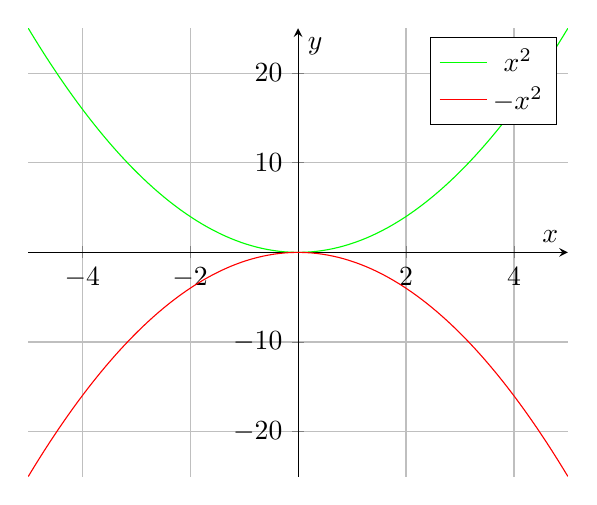
\begin{tikzpicture}
			\begin{axis}[domain=-5:5, axis lines=middle, grid=both, xlabel=$x$, ylabel=$y$, samples=100]
				\addplot[color=green]{x^2};
				\addlegendentry{$x^2$};
				\addplot[color=red]{-x^2};
				\addlegendentry{$-x^2$};
			\end{axis}
		\end{tikzpicture}
	\end{figure}
	\item 
	$
	f_4 :
	\begin{cases}
		\R &\to \R \\
		x &\mapsto f(-x)
	\end{cases}
	$
	\\
	$Gr(f_4)$ se déduit de $Gr(f)$ par symétrie axiale par rapport à l'axe vertical.
	\begin{align*}
		(x,y) \in Gr(f_4) &\iff y = f_4(x) \\
		&\iff y = f(-x) \\
		&\iff (-x, y) \in Gr(f)
	\end{align*}    
	\begin{figure}[h!]
		\centering
		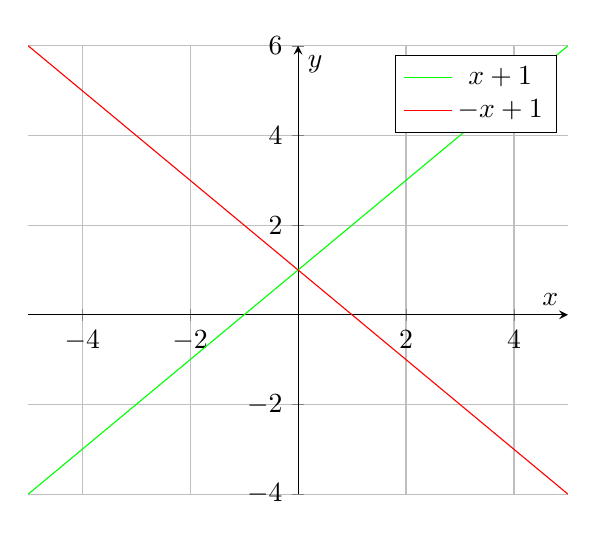
\begin{tikzpicture}
			\begin{axis}[domain=-5:5, axis lines=middle, grid=both, xlabel=$x$, ylabel=$y$, samples=100]
				\addplot[color=green]{x+1};
				\addlegendentry{$x+1$};
				\addplot[color=red]{-x+1};
				\addlegendentry{$-x+1$};
			\end{axis}
		\end{tikzpicture}
	\end{figure}
	\item $f \textnormal{ est paire} \iff Gr(f) \textnormal{ subit une symétrie axiale par rapport à } (O_y)$
	\item $f \textnormal{ est impaire} \iff Gr(f) \textnormal{ subit une symétrie centrale par rapport à l'origine du repère }$
\end{itemize}

% Raphaël Heng
\section{Dérivation}

\begin{graybox}
	\begin{definition}[Dérivabilité]
		\par Soit $I$ un intervalle de $\R$ et $f:I \to \R$. 
		\par On dit que $f$ est \textbf{dérivable}  si $\forall x \in I$
		\begin{align*}
			\lim_{h \to 0}\frac{f(x+h) - f(x)}{h} \textnormal{ existe }
		\end{align*}
		\par On la note $f'(x)$ et $f'$ s'appelle la dérivée de $f$.
		\par Graphiquement $f'(x)$ est la pente de la tangente en $(x, f(x))$ au graphe de $f$.
	\end{definition}
\end{graybox}

\begin{graybox}
	\begin{proposition}[Propriété fondamentale]
		Si $f:I \to \R$ est une fonction dérviable
		\begin{itemize}
			\item $f$ est croissante $\iff f' \geq 0$
			\item $f$ est décroissante $\iff f' \leq 0$
			\item Si $f' > 0$ alors $f$ est strictement croissante
			\item Si $f' < 0$ alors $f$ est strictement décroissante
		\end{itemize}
	\end{proposition}
\end{graybox}

\begin{graybox}
	\begin{proposition}[Formules de dérivation]
		\par Soient $I$ un intervalle et $f,g:I \to \R$ deux fonctions dérivables et $t \in \R$
		\par On a les formules suivantes :
		\begin{itemize}
			\item $(f + g)' = f' + g'$
			\item $(fg)' = f'g + fg'$
			\item $\left(\dfrac{f}{g}\right)' = \dfrac{f'g - fg'}{g^2}$
			\item $(tf)' = tf'$
		\end{itemize}
	\end{proposition}
\end{graybox}

\begin{graybox}
	\begin{proposition}[Dérivation d'une fonction composée]
		\par Soient $I$ et $J$ deux intervalles
		\par Si $f:I \to J$ et $g:J \to \R$
		\begin{align*}
			(g \circ f)' = f' \cdot (g' \circ f)
		\end{align*}
		\par Autrement dit :
		\begin{align*}
			\forall x \in I, (g \circ f)'(x) = f'(x) g'(f(x))
		\end{align*}
	\end{proposition}
\end{graybox}

